\subsection{Overview}
%Electrical overview content here
The power electronics of the Fermion comprises the following subsystems:
\begin{itemize}
    \item Traction Inverter
    \item Precharge and Discharge circuits
    \item Insulation Monitoring Device   
    \item MSD
\end{itemize}

\subsubsection*{Main requirements and design constraints}
\par Our general design of this season is inspired by conventional modes of transportation,
as we have not had the capacity to start developing a levitation system by this season
Thus, we focussed on an electrical system that drives our friction-based motor with
a high amount of acceleration, which is a problem that railway systems frequently face.

\par In between design and production phase, we received a sponsorship of Leadrive,
a local startup for research on automotive power electronics.
Therefore, our workload was eased, which turned out to be favorable
because of our lack of team members in the electrical field. This has been a crucial
constraint in the design and planning process of the electrical department
since the last season. Only shortly before submitting the ITD, we were able to make an estimation of
realistic goals for the new team.

\par This year, we would like to set the path for magnetic levitation in the future, relying on an active system
inside the vehicles. This was taken into consideration when designing the power dimensions,
keeping plenty of overhead for the future, which aligns with our goal of sustainability.
By having reusable modules, the design process of the upcoming years will be simplified.
\begin{figure}[ht]
    \centering
    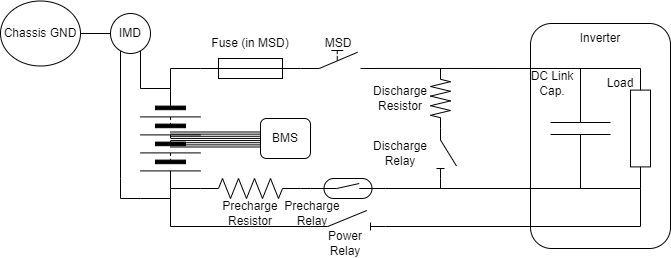
\includegraphics[width=\linewidth]{texfiles/elec/eimg/HVSchematic}
    \caption{Schematic of our power electronics system}
    \label{fig:HVSchematic}
\end{figure}

\subsection{Electrical and mechanical design process}
%Electrical and mechanical design process content here
Our initial goal was to design our own traction inverter system, both the control and power stages. 
After receiving the sponsorship with 
Leadrive, who also sponsors another student team
in Aachen that we collaborate closely with,
we decide to put our own, limited sources to other
projects temporarily. \\
This means that we have a automotive inverter,
with slightly overdimensioned specifications,
to work with. The DC link capacitor of the inverter is charged externally. \\
\subsubsection*{Precharge Circuit}
The precharge circuit was based on an economic decision. Our pod is not made for a commercial purpose. Thus, fast pre-/discharge times are not highly prioritized. We designed with several different precharge resistors at levels from 50 Ohm to 10 kOhm, and simulated them. The results showed that the low-resistance circuits need very high-power components, which will dissipate a lot of heat and be a potential safety danger. However, we wanted to keep the charging times within reasonable times (< 15 seconds), as well as the sizing. As the chassis-mounted precharge resistors rated at 50W were considerably smaller than at 100W, we chose to use them. \\
Deriving from Ohm's law by using the formula for power \(P = U*I\), we get the equation \(R = \frac{U^2}{P} = \frac{500V*500V}{50W} = 5000 \Omega \). Simulating the circuit yielded favorable results. We simulated leaving both relays open for 2 seconds, then charging the capacitor with a 5k resistor for 8 seconds, then switching to the main power line by opening the respective relays. Due to financial reasons (due to the lack of available 5k resistors), we changed the value to 4.7k, which gave us many more favorable candidates. A quick estimation with \(\sqrt{R*P} = \sqrt{4700\Omega*50W} = 484.77V\) shows that this is still above our nominal voltage. Furthermore, we chose a resistor that can handle overpower for short amount of times (refer to final system description).  At all time, the power ratings were abided as seen in the chart.  \\
The objects of the simulation are as follows: 
\begin{itemize}
    \item C1: DC Link Capacitor
    \item R1: Precharge Resistor
    \item V2: Battery
    \item S1: Precharge Relay
    \item n003: positive wire of capacitor
    \item V(N003,N002)*I(R1): Power through the resistor
    \item V(N003)*I(C1): Power through the capacitor
    \item V(N002)*I(V2): Power through the battery
\end{itemize}
    
\begin{figure}[ht]
    \centering
    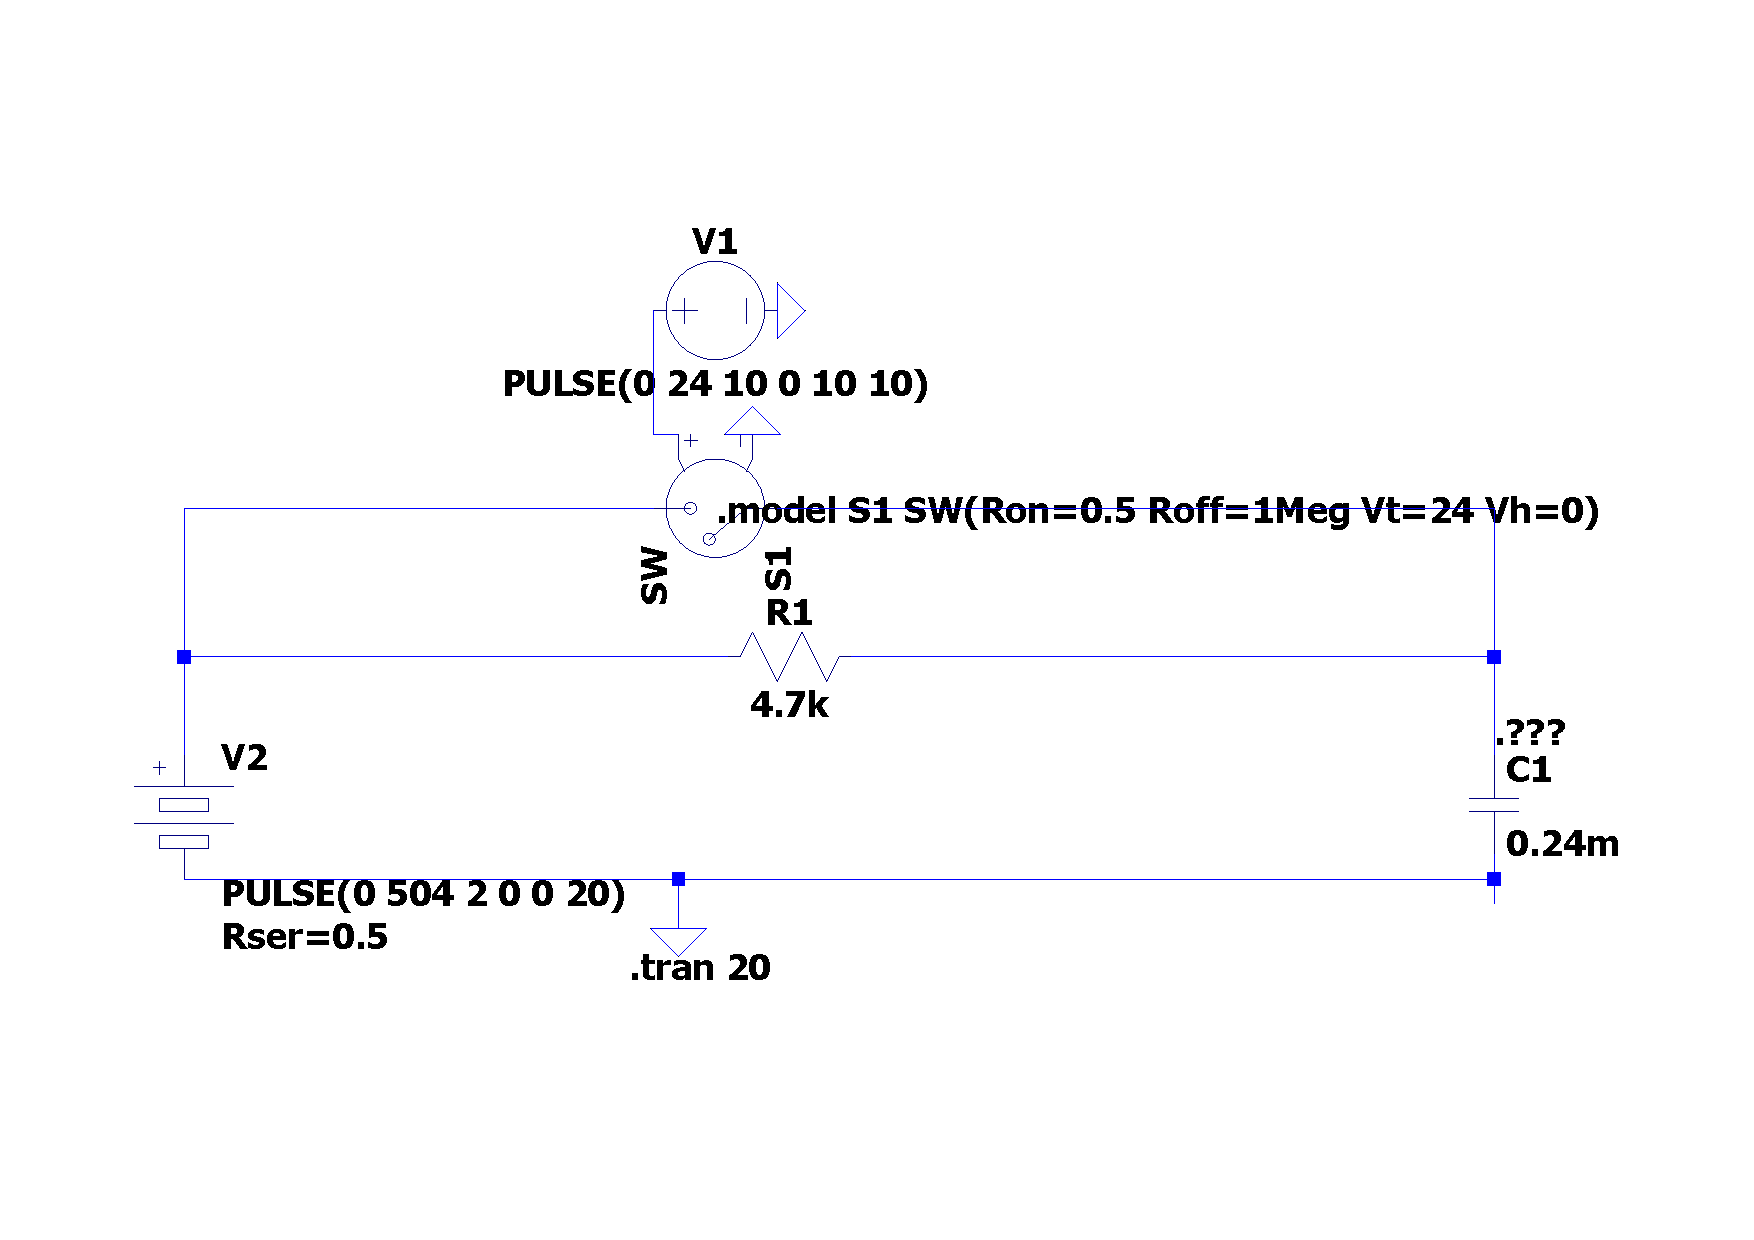
\includegraphics[width=\linewidth]{texfiles/elec/eimg/PrechargeCircuit}
    \caption{Precharge Circuit Schematic with 4.7k Resistor}
    \label{fig:PrechargeCircuit}
\end{figure}

\begin{figure}[ht]
    \centering
    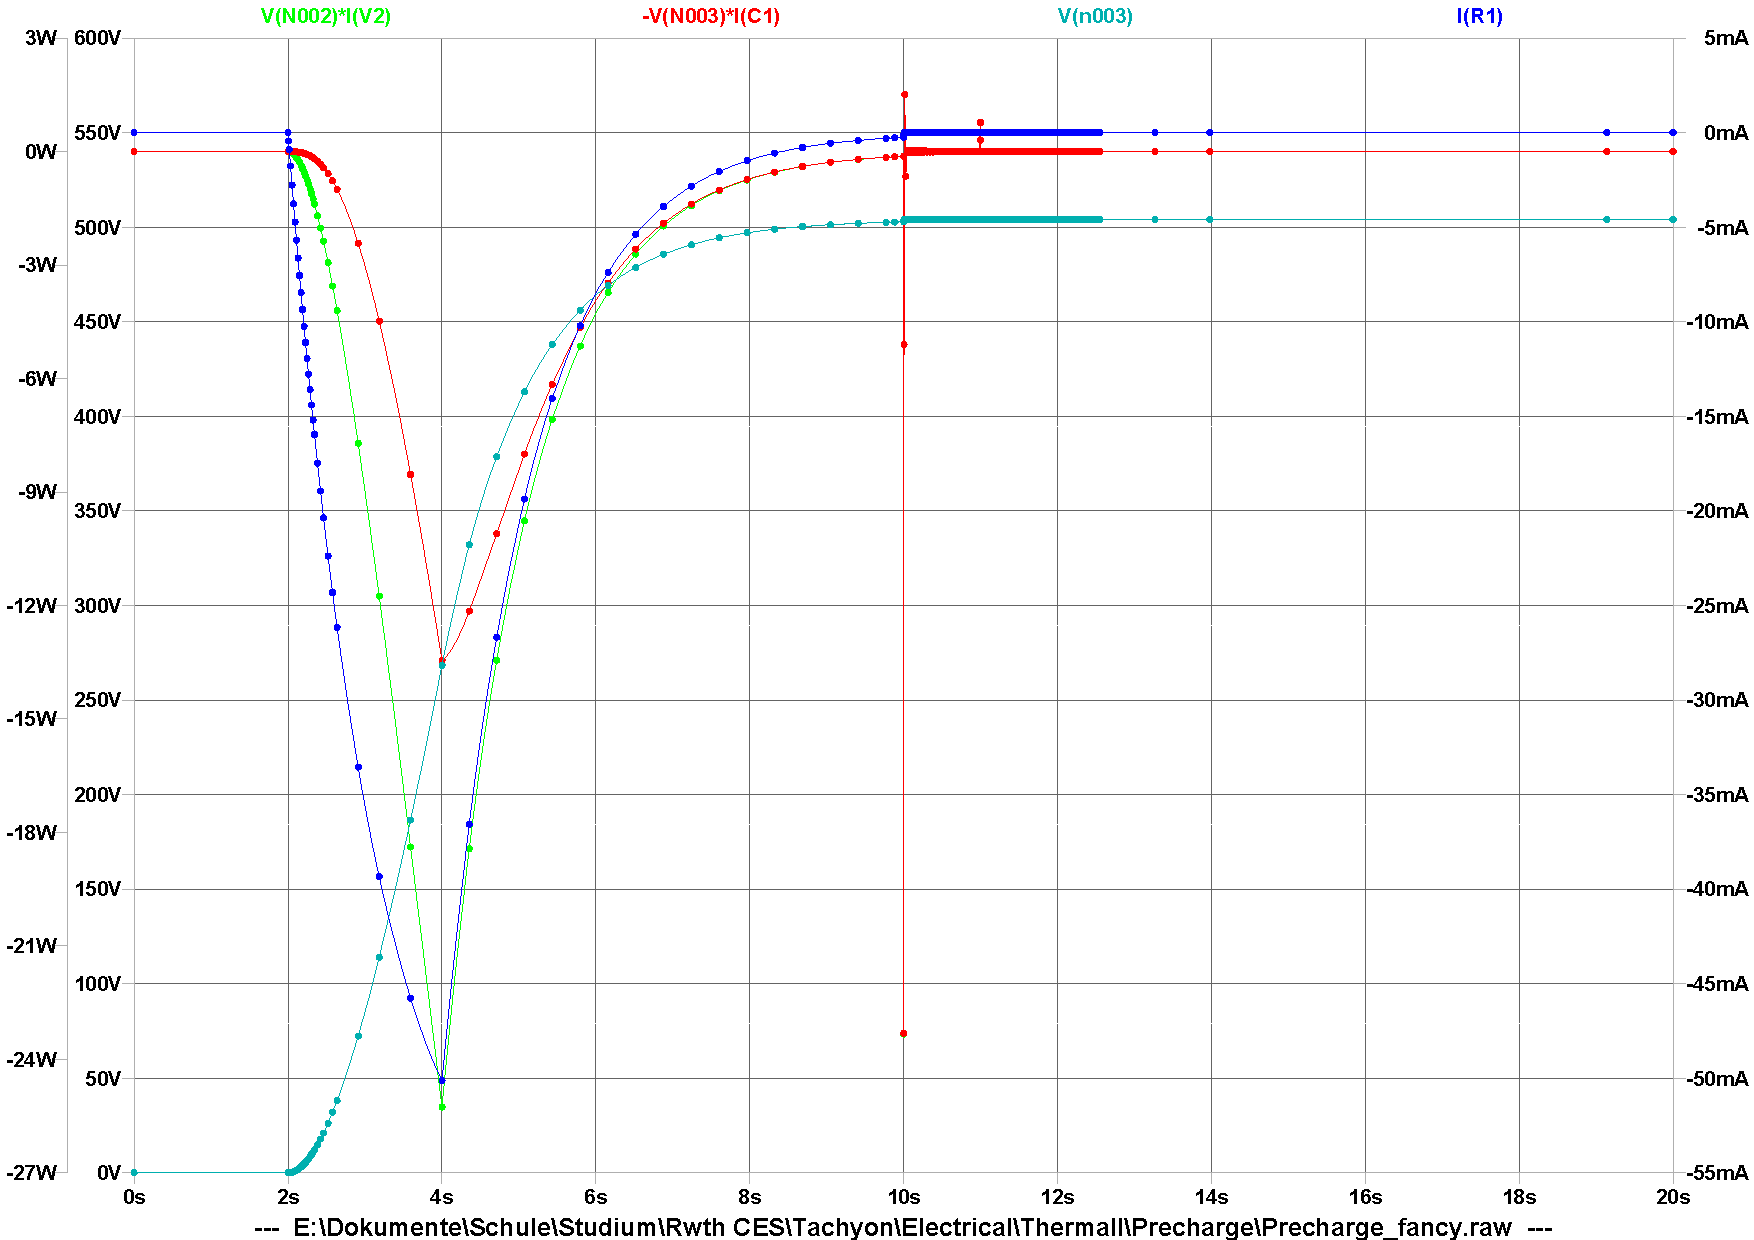
\includegraphics[width=\linewidth]{texfiles/elec/eimg/PrechargeSimulation4.7k}
    \caption{Precharge Circuit Simulation with 4.7k Resistor}
    \label{fig:PrechargeSimulation4.7k}
\end{figure}

This gives us the following specifications of our precharge circuit:
\begin{itemize}
\item Time Constant (\( \tau \)):
\[ \tau = R \times C = 4700 \, \Omega \times 0.24 \times 10^{-3} \, \text{F} = 1.128 \, \text{s} \]

\item Voltage across the capacitor at \( t = 8 \) seconds:
\[ V(8) = 504 \times \left(1 - e^{-\frac{8}{1.128}}\right) = 503.58V, \Delta V = 0.42V \]
\end{itemize}
In our simulations, we see that the power through the circuit when switching to the main valve at t = 10s is not higher than 35 Watts, which is perfectly acceptable.

\subsubsection*{Discharge Circuit}
It is convenient and advantegeous to use a discharge circuit when shutting of the system, tackling the safety hazard of a charged HV DC Link capacitor. We use the same resistor to discharge the capacitor. The peak power through the resistor is \( \frac{504^2}{5000} = 50W \), . The time constant is \( \tau = 5k \Omega \times 0.24 \times 10^{-3} \, \text{F} = 1.2s \). This means that the capacitor is discharged to 1\% of its voltage after 12 seconds. This is acceptable and in accordance with the recommendation of the producing company, Leadrive, who suggests a minimum of 4 seconds.

\subsubsection{Present Schematics or logic diagrams of the boards.}

We are not allowed to disclose information about the traction inverter, as it is an OEM product. We will treat it like a black box device. 
The same goes for the insulation monitoring device.
\subsubsection{(b) Present temperature simulations for vacuum conditions.}
For our heat simulations, we used the software of ANSYS. By vacuum conditions, we assumed the
lack of gas flow, which eliminates the cooling heat flow from winds. The simulation tool solves
the heat transfer equation \( \frac{\partial T}{\partial t} = \alpha \left( \frac{\partial^2 T}{\partial x^2} + \frac{\partial^2 T}{\partial y^2} + \frac{\partial^2 T}{\partial z^2} \right) \)
by discretizing through Finite-Element-Methods.
\begin{figure}[H]
    \centering
    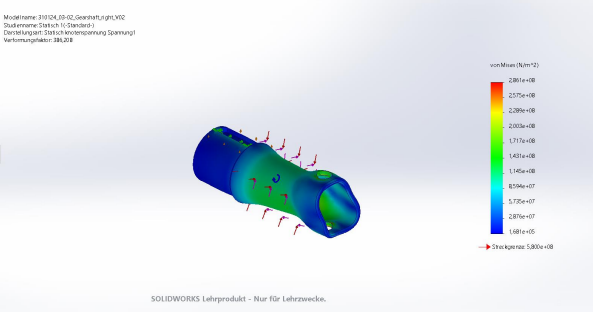
\includegraphics[width=0.9\textwidth]{texfiles/elec/eimg/SimulationTemplate}
    \caption{Simulation results}
    \label{img: simresults_battery}
\end{figure}


\subsection{Description of subsystem control}
%Description of subsystem control content here
\subsubsection{(a) Briefly reference the control systems of the boards, which should be explained in the levitation or propulsion subsection respectively.}
The precharge and discharge circuits are controlled via the relays. That is possible throough the Raspberry Pi 4 of the telemetry system, which also handles the CAN communication with the inverter of Leadrive.


\subsection{Electrical system characteristics}   
\begin{table}[H]
    \centering
    \begin{adjustbox}{width=\textwidth,center}
    \begin{tabular}{|l|c|c|c|l|l|}
        \hline
        \textbf{Parameter} & \textbf{MIN} & \textbf{NOM} & \textbf{MAX} & \textbf{Unit} & \textbf{Conditions} \\
        \hline
        Ambient Temp. for Operation ($T_{\text{AMB}}$) & -40 & - & 90 & °C & - \\
        \hline
        Ambient Temp. for Storage ($T_{\text{STO}}$) & -40 & - & 85 & °C & - \\
        \hline
        Relative Humidity & 0 & - & 95 & \% & - \\
        \hline
        Flow Rate of Coolant ($V_{\text{CLNT}}$) & 8 & 12 & 16 & l/min & Derating @ $8\sim12$ l/min \\
        \hline
        Inlet Temp. of Coolant ($T_{\text{CLNT}}$) & -40 & - & 85 & °C & Derating @ $65\sim85$°C \\
        \hline
        Cooling Inlet Pressure ($P_{\text{INLET}}$) & - & - & 2.5 & bar & - \\
        \hline
        Pressure Drop between Cooling Inlet and Outlet ($P_{\text{DROP}}$) & - & 0.25 & - & bar & $T_{\text{CLNT}}=65°C$, $V_{\text{CLNT}}=12$ l/min \\
        \hline
        Input Voltage ($V_{\text{DC}}$) & 260 & 600 & 850 & V & Full operation @ $450-800$V \\
        \hline
        Input Current ($I_{\text{DC}}$) & - & 200 & - & A & Continuous \\
        \hline
        Peak Input Current ($I_{\text{DCPK}}$) & - & 300 & - & A & For max $t_{\text{PK}}$ duration \\
        \hline
        Output Voltage ($V_{\text{AC}}$) & - & 400 & - & Vrms & - \\
        \hline
        Output Current ($I_{\text{AC}}$) & - & - & 200 & Arms & Continuous \\
        \hline
        Peak Output Current ($I_{\text{ACPK}}$) & - & - & 300 & Arms & For max $t_{\text{PK}}$ duration \\
        \hline
        Output Power ($S_{\text{AC}}$) & - & 135 & - & kVA & Continuous \\
        \hline
        Peak Output Power ($S_{\text{ACPK}}$) & - & 200 & - & - & For max $t_{\text{PK}}$ duration \\
        \hline
        Peak Duration ($t_{\text{PK}}$) & - & - & 60 & s & - \\
        \hline
        Input Voltage for Control ($V_{\text{BAT}}$) & 6 & - & 36 & V & Full functional @ $8-32$V (control board) \\
        \hline
        Max. Efficiency ($\eta$) & 97 & - & - & \% & - \\
        \hline
        Torque Control Accuracy ($\epsilon_{\text{TRQ}}$) & - & - & 3 & \% & Torque $>100$Nm \\
        \hline
         & - & - & 3 & Nm & Torque $<100$Nm \\
        \hline
        Torque Control Speed ($t_{\text{TRQ}}$) & - & - & 100 & ms & - \\
        \hline
        Speed Control Accuracy ($\epsilon_{\text{SPD}}$) & - & - & 30 & rpm & - \\
        \hline
    \end{tabular}
    \end{adjustbox}

    \caption{800V Single Inverter Specifications}
    \label{inverter_specs}
\end{table}

\subsection{Interface with other system}
%Interface with other system content here n
(a) Briefly reference the communication protocols or control mechanisms of the boards, which should be explained in the respective Sense and Control subsection. \\
All the electric subsystems are located within the pod. \\

The phsyical connection matrix is as following:
\begin{table}
    \centering
    \begin{adjustbox}{width=\textwidth,center}
    \begin{tabular}{|c|c|c|c|c|c|c|}
    \hline
    From | To & \text{LV Battery} & \text{HV Battery} & \text{BMS} & \text{Traction Inverter} & \text{Motor} & \text{Cooling System} \\
    \hline
    \text{LV Battery} & - & - & Powers & \text{Powers control system} & - & \text{Powers pump and control system} \\
    \hline
    \text{HV Battery} & - & - & Connects to & \text{Provides power} & - & - \\
    \hline
    \text{BMS} & - & - & \text{Controls} & - & - & - \\
    \text{Traction Inverter} & - & - & - & - & \text{Propels} & X \\
    \hline
    \text{Motor} & - & - & - & - & - & - \\
    \hline
    \text{Cooling System} & - & - & - & \text{Cooling} & \text{Cooling} & \text{Cooling (implicitly)} \\
    \hline
    \end{tabular}
\end{adjustbox}
\caption{Physical connection matrix}
\label{Physical connection matrix Power}
\end{table}

The data connection matrix is as following. All communication between boards are via CAN, if not specified otherwise:

\begin{table}
    \centering
    \begin{adjustbox}{width=\textwidth,center}
    \begin{tabular}{|l|c|c|c|c|c|c|c|c|}
    \hline
    From $\backslash$ To & LV Battery & HV Battery & BMS & Traction Inverter & Motor & Cooling System & Brakes Controller & Telemetry Unit  \\
    \hline
    LV Battery & - & - & - & - & - & - & - & - \\
    HV Battery  & - & - & Discharge rate, voltage level & - & - & - & - & - \\
    BMS & controls & controls & - & - & - & - & - & sends data \\
    Traction Inverter & - & - & - & - & - & - & - & sends data \\
    Motor & - & - & - & - & - & - & - & - \\
    Cooling System & - & - & - & - & - & - & - & sends data \\
    Brakes Controller & - & - & - & - & - & - & - & sends data \\
    Telemetry Unit & - & - & updates limits & sends commands & - & sends target rates & sends commands & - \\
    \hline
    \end{tabular}
    \end{adjustbox}
    \caption{Data connection matrix}
    \label{data-connectivity-matrix-power}
\end{table}


\subsection{Final system description}
Parts List: \\




\subsubsection*{Precharge and Discharge Circuit}
We have a precharge circuit and discharge circuit for the DC Link Capacitor during the startup/shutdown phase to deal with the empty/charged capacitor. The design can be seen in \href{fig:HVSchematic}{this figure from above}.
We utilize the following \href{tab:precharge-relay-specs}{relay}: KT24-1A-40L-THT from Meder electronic and the following \href{tab:precharge-resistor}{resistor} WH50-4K7JI from TT Electronics.

\begin{table}[h] 
\begin{tabular}{|l|c|}
    \toprule
    Parameter & Value \\
    \midrule
    Model &  WH50-4K7JI \\
    Company & TT Electronics \\
    Power Rating at 25°C & 50 W \\
    Resistance Range & 4.7K Ohms \\
    TCR (-55° to 200°C) for ≥10R & ±25 ppm/°C \\
    Resistance Tolerance Options & ±5\% \\
    Isolation Voltage & 3000 V DC or AC peak \\
    Operating Temperature Range & -55 to +250°C \\
    \bottomrule
\end{tabular}
\label{tab:precharge-resistor}
\caption{Precharge (and Discharge) Resistor Specifications}
\end{table}

\begin{table}[H]
    \centering
    \begin{tabular}{|l|c|c|c|c|}
    \hline
    \textbf{Parameter} & \textbf{Min} & \textbf{Typ} & \textbf{Max} & \textbf{Unit} \\
    \hline
    Coil Resistance & 1.620 & 1.800 & 1.980 & Ohm \\
    Coil Voltage & & 24 & & VDC \\
    Rated Power & & 320 & & mW \\
    Thermal Resistance & & 80 & & K/W \\
    Inductance & & 430 & & mH \\
    Pull-In Voltage & & & & VDC \\
    Drop-Out Voltage & 2.9 & & 16 & VDC \\
    Contact Rating & & & 100 & mA \\
    Switching Voltage & & & 1.000 & V \\
    Switching Current & & & 1 & A \\
    Carry Current & & & 2.5 & A \\
    Contact Resistance Static & & 150 & 200 & mOhm \\
    Contact Resistance Dynamic & & & & mOhm \\
    Insulation Resistance & 10 & & & GOhm \\
    Breakdown Voltage (40-50 AT) & 3 & & & kV DC \\
    Capacitance & & & 0.5 & pF \\
    Dielectric Strength Coil/Contact & & & 7 & KV DC \\
    Dielectric Strength Contact/Contact & & 1.2 & & KV DC \\
    Housing Material & & & & \\
    Approvals & & & yes & \\
    \hline
    \end{tabular}
    \caption{Precharge/Discharge Relay Specifications}
    \label{tab:precharge-relay-specs}
\end{table}


\subsubsection{Insulation Monitoring Device}
The Insulation Monitoring Device that is mandatory for EHW participants, as well as Formula Students teams, is not built inhouse, after receiving the respective advice from the EHW technical jury. By reaching out to Bender, we received their device (Bender A-ISOMETER ® iso-F1 IR155-3204) through their Formula Students program. This device was approved for the FSE competitions. It is configured for a responding insulation resistance value of 500 kOhm between HV+ and Chassis, and between HV- and Chassis, following the guidance of approx. \(500 \frac{\Omega}{V}\). This takes into account that we might increase the dimension of our system in future designs. The calculation takes place with a DCP factor of 10, meaning that the detection value is calculated out of the mean of 10 measurements, which was suggested by the manufacturer.\\
Furthermore, we have the IMD set to detect undervoltage at 400V, which helps us do detect serious malfunctioning. This is a redundant feature that is also handled by the BMS. We do not expect our battery pack to ever fall under 400V. \\
The device is certified according to ISO16750. It will trigger a LED when there is no leak. Furthermore, we will read its outputs, which are a PWM signal, and a status binary output showing the proper working. Both the duty cycle and the frequency of the PWM contain relevant information. Both outputs furthermore require 2.2kOhm pull-down resistors. \\
\begin{table}[H]
    \centering
    \caption{Insulation Monitoring Device Specifications}
    \label{tab:table1}
    \begin{adjustbox}{width=\textwidth}
    \begin{tabular}{|l|l|}
        \hline
        \textbf{Parameter} & \textbf{Specification} \\
        \hline
        Protective separation & Between (L+/L-) – (Kl. 31, Kl. 15, etc.) \\
        Voltage test & AC 3500 V/1 min \\
        Supply voltage \(U_S\) & DC 10 V…36 V \\
        Max. operating current \(I_S\) & 150 mA \\
        Max. current \(I_k\) & 2 A \\
        Inrush current & 6 A/2 ms \\
        HV voltage range (L+/L-) \(U_n\) & AC 0 V…1000 V (peak value) \\
        & 0…660 V r.m.s. (10 Hz…1 kHz) \\
        & DC 0 V…1000 V \\
        Power consumption & < 2 W \\
        Response value hysteresis (DCP) & 25 \% \\
        Response value \(R_{an}\) & 100 kΩ…1 MΩ \\
        Undervoltage detection & 0 V…500 V \\
        Load dump protection (-32xx) & < 60 V \\
        Load dump protection (-42xx) & < 50 V \\
        Measurement method & Bender-DCP technology \\
        Factor averaging \(F_{ave}\) (output M) & 1…10 (factory set: 10) \\
        ESD protection, contact discharge   & ≤ 10 kV (to terminals)\\
        ESD protection, contact discharge  & ≤ 25 kV (indirectly to environment) \\
        ESD protection (air discharge – handling of the PCB) & ≤ 6 kV \\
        \hline
    \end{tabular}
    \end{adjustbox}
\end{table}

\subsubsection*{Overcurrent Protection and MSD}
We buy the manual safety disconnect from Amphenol (Amphenol MSDM6302 + Amphenol MSDF000R). This MSD can be opened without removing any parts of the Fermion as it is accesible by opening a lid of the shell. It can be opened with one hand and is rated for a temperature between -40°C and 70°C. There is a fuse built in the MSD. It is rated for 630A and 690V. The manufacturer recommends that the current be a third of the rated fuse current, which is \(630A/3 = 210A\). \footnote{\href{https://www.amphenol-industrial.de/de/amph/download/viewFile/MTA0}{Product Sheet EXCEL|MATE MSD
Manual Service Disconnect}, Amphenol PCD Shenzhen} \\


\subsection{Manufacturing process}
%Manufacturing process content here
Our PCB Design
\subsubsection{PCBs}
\par Prototyping: Prototype PCBs are fabricated in the FabLab associated with our university. The FabLab provides access to PCB manufacturing equipment and materials, enabling the rapid production of prototypes for initial testing and design validation.
    Once the PCBs are fabricated, they are assembled manually by our team members. 
\par Production: We ordered our final PCBs from JLCPCB, a leading PCB manufacturing service. In addition to JLCPCB, we also collaborate with Würth Elektronik who produce 
PCBs in Germany, aligning with our goal of sustainability.

\subsubsection{Inverter}
The inverter is a product from Leadrive used as an OEM product in automotive and mobility industry. \\

    Support from Leadrive: The development of the inverter system is supported by Leadrive, a company specializing in advanced inverter technology. Their expertise significantly contributes to the optimization of our propulsion system.
    Collaboration with Formula Student Team of FH Aachen: Additionally, we collaborate with the Formula Student Team of FH Aachen, benefiting from their practical experience in electric vehicle design and inverter application. This partnership enriches our project with valuable insights into inverter integration and performance enhancement.

\subsection{Testing}
%Testing content here
We started testing software.

%\subsection{FMEA}
%FMEA content here
